\documentclass{jsarticle}
\usepackage{graphicx, listings, jlisting, xcolor, colortbl}
\lstset{%
  language=Verilog,
  belowcaptionskip=1\baselineskip,
  breaklines=true,
  frame=L,
  xleftmargin=\parindent,
  showstringspaces=false,
  basicstyle=\footnotesize\ttfamily,
  keywordstyle=\bfseries\color{green!40!black},
  commentstyle=\itshape\color{purple!40!black},
  identifierstyle=\color{blue},
  stringstyle=\color{orange},
}
\title{情報実験第三 課題2}

\author{15\_03602 柿沼 建太郎 \\ 情報工学科 15\_10588 中田 光}
\date{\today}
\begin{document}
\maketitle

\section*{作成したプログラムの概要}
今回の課題では、課題1で作成された電卓プログラムの改造を行った。
Verilogコードの改変とEX3のコードの改変をともに行った。
追加・変更する予定であった機能は以下の通り。
\subsection*{Verilogコードの追加/変更}
\begin{itemize}
    \item CPUの32bit化
    \item 命令数の追加
    \item 固定小数を実装
    \item メモリ参照命令を追加(減算,乗算,除算,剰余)
\end{itemize}
\subsection*{EX3コードの追加/変更}
\begin{itemize}
    \item 小数の入力受付
    \item 表示の10進化
    \item 乗算,除算,剰余,平方根などの新たな演算の実装
\end{itemize}
しかしこの内「減算・剰余命令の追加」と「固定小数の実装」及びそのソフトウェア側での対応は時間が足りず間に合わなかった。

\section*{各作業の担当者}
\begin {table}[h]
    \begin {tabular}{|c|c|} \hline
        \rowcolor[rgb]{0.85, 1.0, 1.0} 作業名 & 担当者 \\ \hline
        CPUの32bit化 & 柿沼 \\ \hline
        命令数の追加 & 柿沼 \\ \hline
        メモリ参照命令の追加 & 柿沼 \\ \hline
        小数の入力受付 & 中田 \\ \hline
        表示の10進化 & 中田 \\ \hline
        乗算,除算,剰余,平方根などの新たな演算の実装 & 中田 \\ \hline
    \end {tabular}
\end {table}

\section*{Verilogコードの追加/改変}
担当者 柿沼

\subsection*{CPUの32bit化}
与えられたVerilogコードで実装されたCPUは16bitCPUであったが、固定小数による計算をするにあたって16bitでは精度が足りないと判断し、ACレジスタなどの容量を32bitまで拡張した。
具体的には以下のように改変した。
\begin {itemize}
    \item ALUの32bit計算対応
    \item RAMとROMの32bit化
    \item DR,ACレジスタの容量の32bit化
    \item バス容量の32bit化
\end {itemize}
前回の課題でACレジスタの中身を7セグメント表示用レジスタに転送する命令を作成したが、7セグメントディスプレイには16bitぶんしか表示できなかったため、下位16bitのみしか表示されていない。
LEDでの表示についても同様の対処がされている。
また、与えられたEX3シミュレータは出力するファイルが16bitのデータとなっていたため、32bit出力するように対応した。

\subsection*{命令数の追加とメモリ参照命令の追加}
掛け算命令や割り算命令などを追加したほうがソフトウェア側での高機能な計算が楽になると思い、Verilogコード側で実装することにした。
具体的にはメモリ参照命令で掛け算と割り算を行う「MUL」と「DIV」を実装した。
掛け算や割り算命令はメモリ参照命令でありオペコードに空きがなかったため、オペコードを16bitから17bitに変更した。
オペコードの割り当てについては変更を最小限にするためにIRレジスタの16,14,13,12bit目の計4bitを見て命令種別を判別することとした。
そのため掛け算命令「MUL」のオペコードは10XXXと18XXX、割り算命令「DIV」のオペコードは11XXXと19XXXとなっている。

\section*{感想}
柿沼

CPUの32bit化の作業中にバグが大量に発生し、ほとんどその対応に時間を使ってしまった。
数字を変えるだけだと侮っていたと思う。
結局何度か修正していたら直ったが、原因はよくわからなかった。
命令の拡張などはすぐにできたので、バグが大量発生した時点で早めに打ち切り、固定小数の実装に移っておくべきだったと今では思う。
固定小数の実装が間に合わなかったため根号計算などが作れなかったのが痛手だと感じる。
また、Verilogシミュレータをうまく使いこなせなかったのも時間のロスの原因だと思う。
入出力の部分が見にくかったので結局ほとんどのデバッグをFPGAでやっていたのだが、ビルドに時間が掛かる上に授業中しかデバッグができない。Verilogシミュレータを使いこなせばもう少し効率的に作業ができたのではないかと思う。

\section*{test\_calc1の機能拡張:ソフトウェアプログラム}
担当:中田\\
\subsection*{概要}
計算機プログラムのアセンブリコードtest\_calc1.asmを改良し、入出力の10進数化、計算機能の拡張を行った。
計画当初では固定小数を実装する予定であったが、ハードウェアとソフトウェアの双方で完成の目途が立たず、残された日数を考慮し、
今回は実装を断念した。それに伴い実装予定だった平方根の機能拡張についても整数値しか扱うことができず、ニュートン法を用いた方法では
精度が期待できなかったため他の計算機能を拡張した。以下に拡張した機能と主なラベルを記す。また、入力は全て中置記法で入力する。

\begin{table}[h]
  \begin{tabular}{|l|p{10cm}|} \hline
    機能 & 機能の説明 \\ \hline
    乗算 & 乗算を計算する。演算子は'*'。 \\ \hline
    除算 & 除算を計算する。剰余は切り捨て。演算子は'/'。 \\ \hline
    指数計算 & 指数計算をする。演算子は'\^{}'。 \\ \hline
    組み合わせ & 組み合わせを計算する。演算子は'c'。 \\ \hline
    総乗 & P\_YからP\_Xまでの積を計算する。$x p 1 =$とするとxの階乗の計算となる。演算子は'p'。 \\ \hline 
  \end{tabular}
\end{table}

\begin{table}[h]
  \begin{tabular}{|l|p{10cm}|} \hline
    ラベル & ラベルの説明 \\ \hline
    READ\_DX & 入力が0~9かを判断する。 \\ \hline
    H2D & Zの16進の値を出力用のレジスタZHMGに10進数で格納する。	\\	\hline
    P & 総乗を計算をする。$\prod_{i=P\_Y}^{P\_X} i$をP\_RESに格納する。 \\ \hline
    C & 組み合わせを計算をする。${}_{P\_X}C_{P\_Y}$をP\_RESに格納する。 \\ \hline
    EXP & 指数を計算する。${EXP\_X}^{EXP\_Y}$をEXP\_RESに格納する。 \\ \hline 
  \end{tabular}
\end{table}

\newpage

\subsection*{実行結果}

\begin{figure}[htbp]
 \begin{minipage}{0.5\hsize}
  \begin{center}
  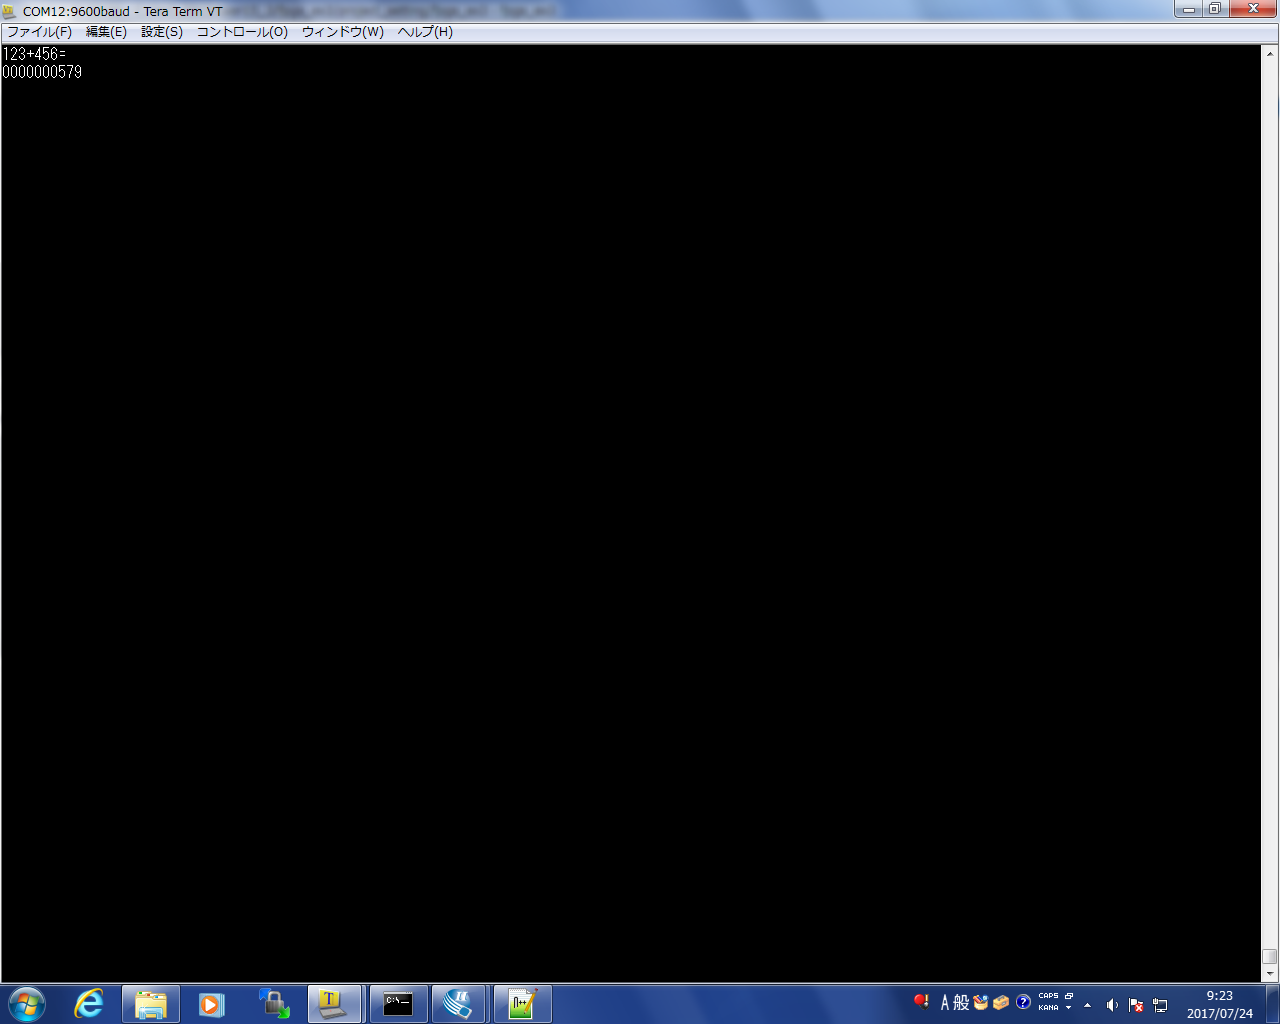
\includegraphics[width=8cm,bb=0 0 1280 1024]{123+456.png}
  \end{center}
  \caption{"$123+456=$"}
 \end{minipage}
 \begin{minipage}{0.5\hsize}
  \begin{center}
   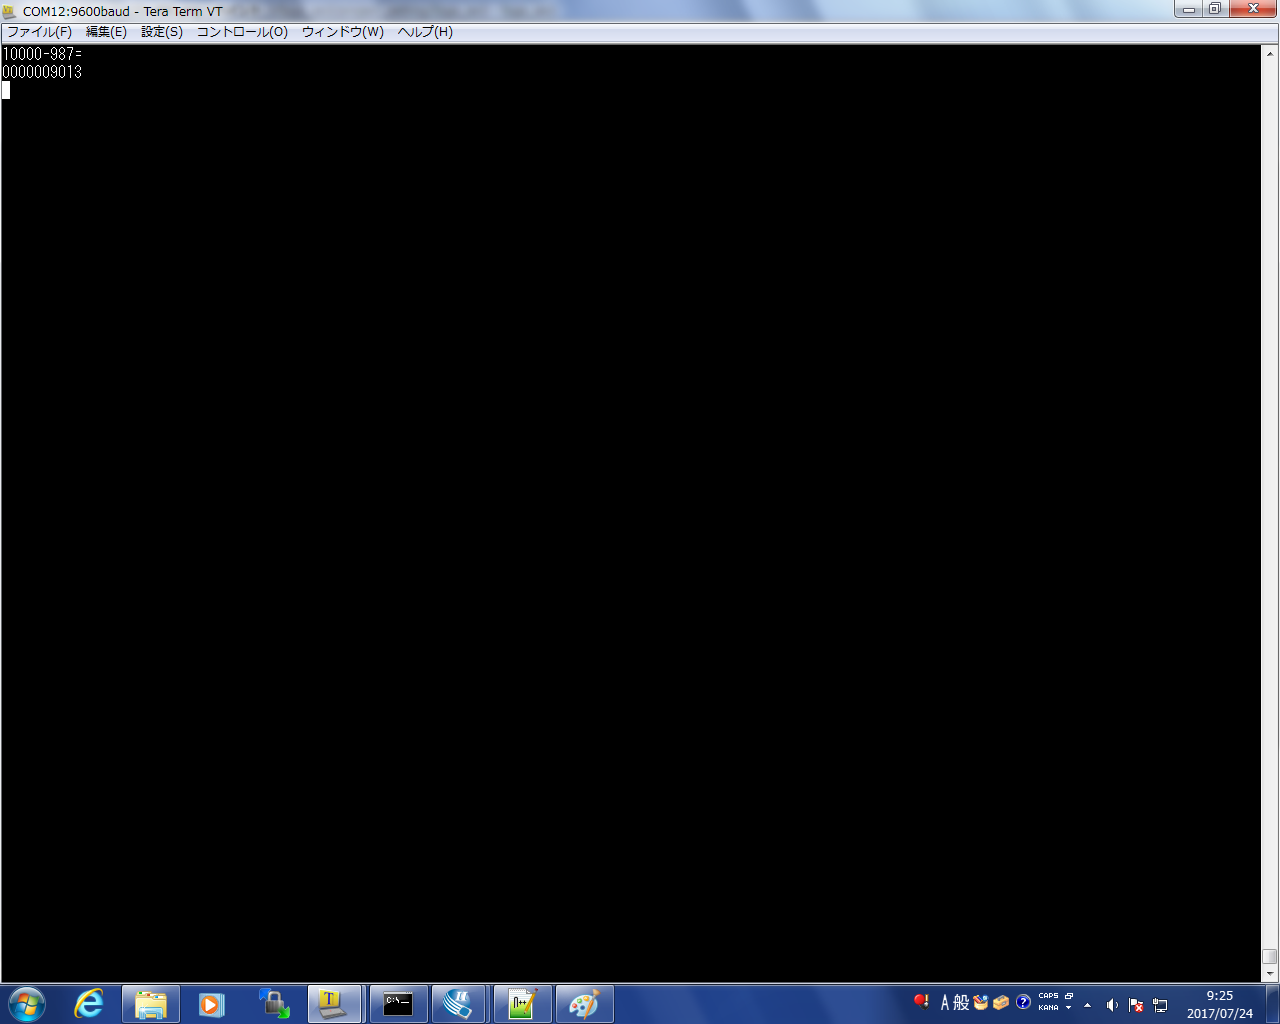
\includegraphics[width=8cm,bb=0 0 1280 1024]{10000-987.png}
  \end{center}
  \caption{"$10000-987=$"}
 \end{minipage}
\end{figure}

\begin{figure}[htbp]
 \begin{minipage}{0.5\hsize}
  \begin{center}
  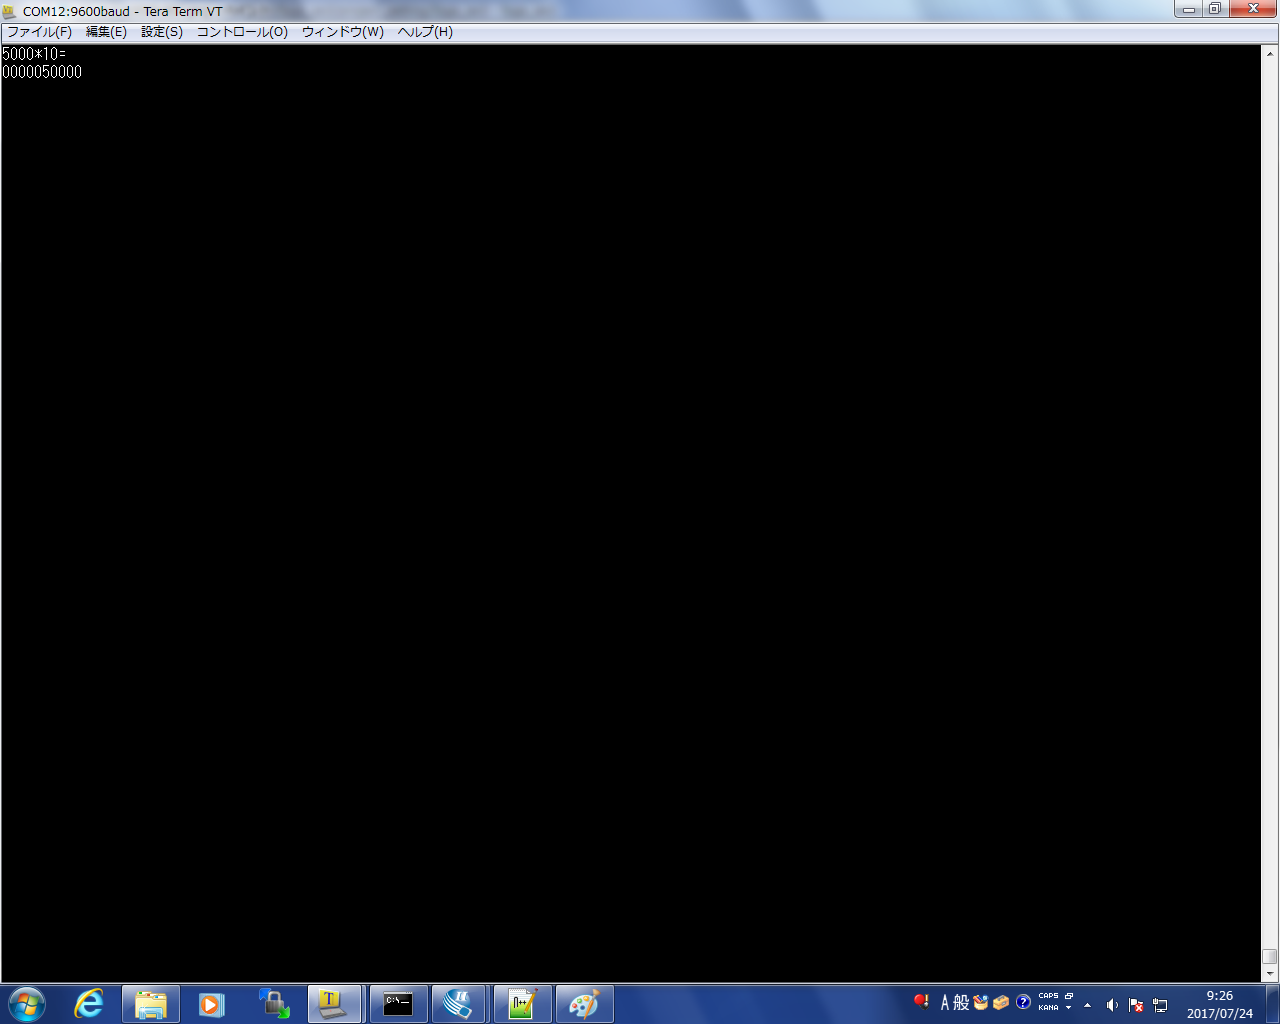
\includegraphics[width=8cm,bb=0 0 1280 1024]{5000mul10.png}
  \end{center}
  \caption{"$5000\times10=$"}
 \end{minipage}
 \begin{minipage}{0.5\hsize}
  \begin{center}
   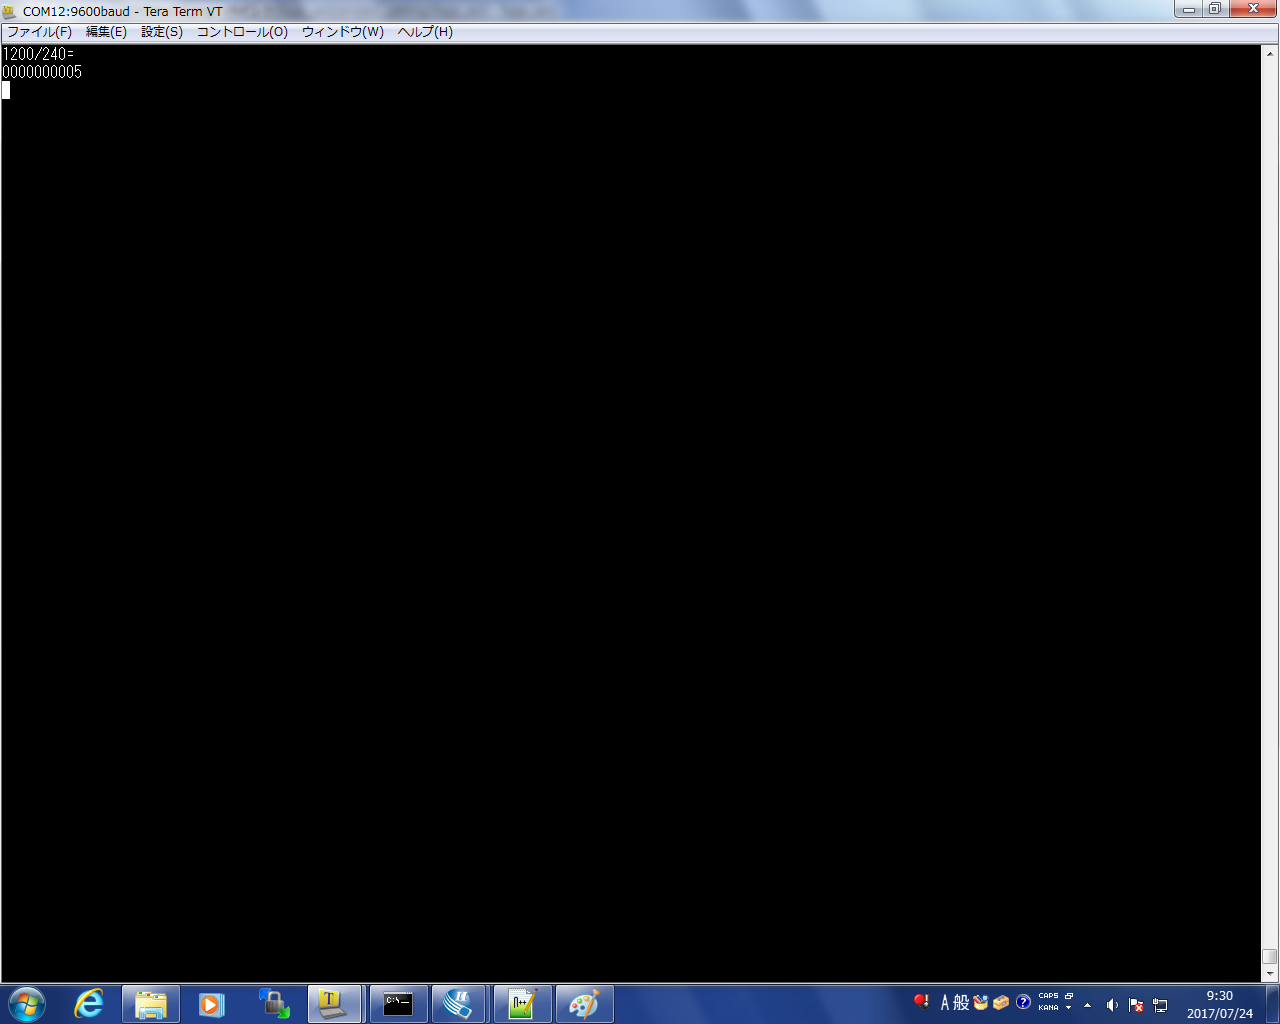
\includegraphics[width=8cm,bb=0 0 1280 1024]{1200div240.png}
  \end{center}
  \caption{"$1200\div240=$"}
 \end{minipage}
\end{figure}


\begin{figure}[htbp]
 \begin{minipage}{0.5\hsize}
  \begin{center}
  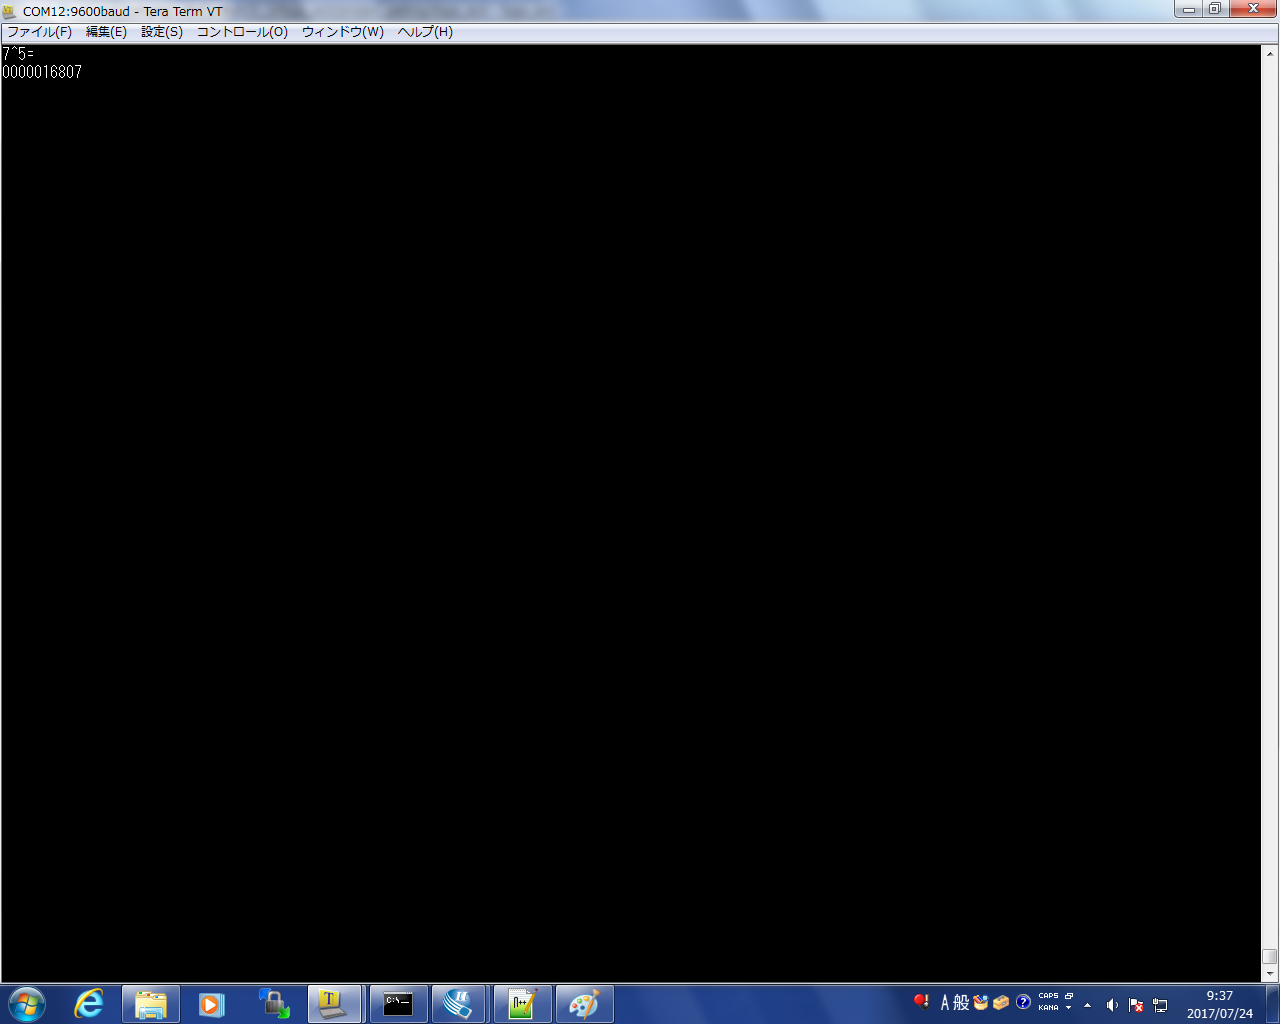
\includegraphics[width=8cm,bb=0 0 1280 1024]{7^5.png}
  \end{center}
  \caption{"$7^5=$"}
 \end{minipage}
 \begin{minipage}{0.5\hsize}
  \begin{center}
   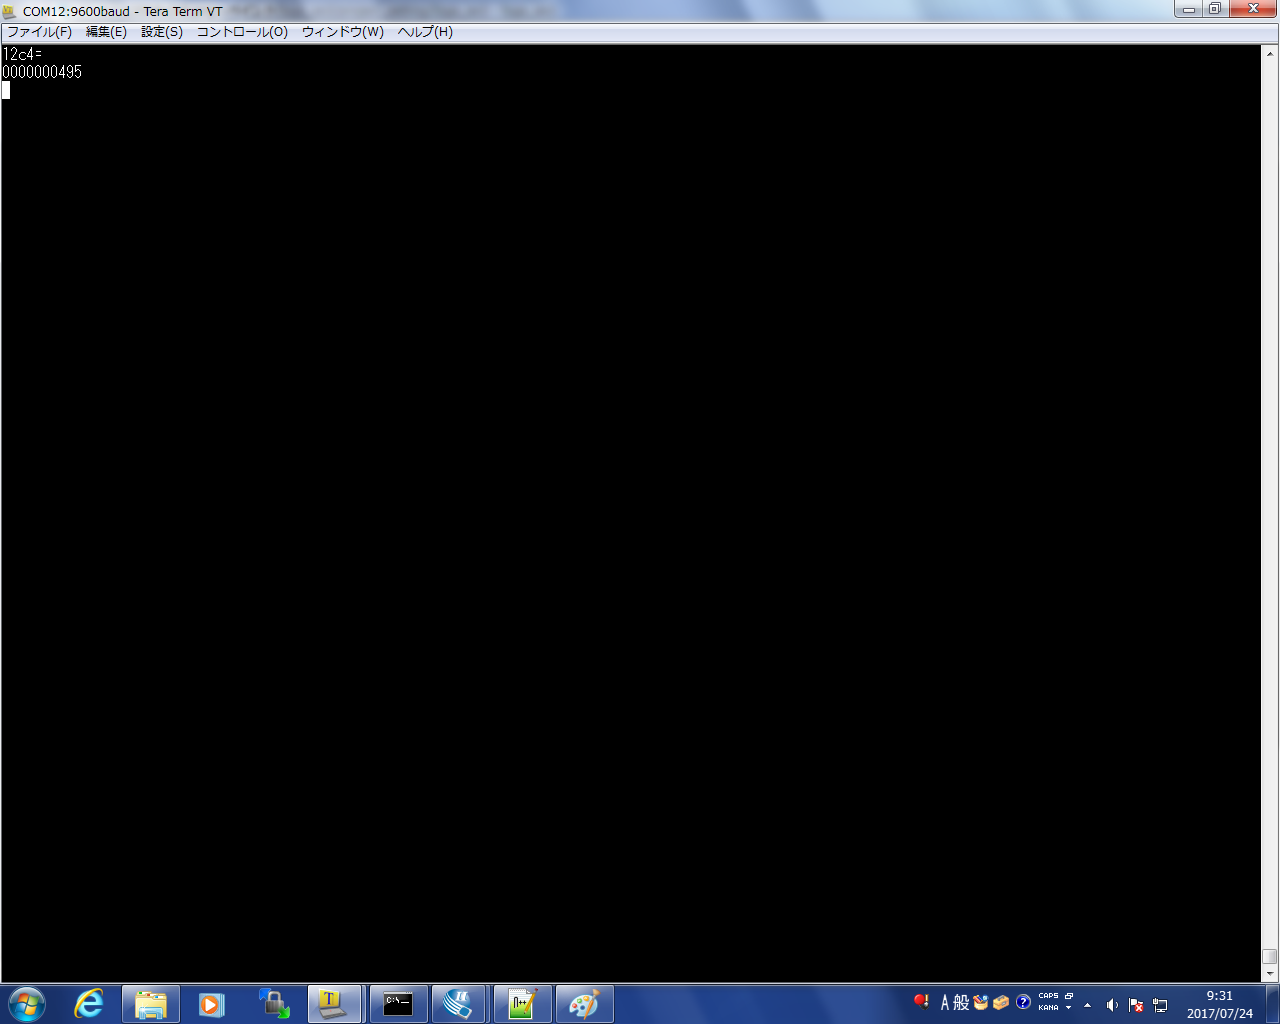
\includegraphics[width=8cm,bb=0 0 1280 1024]{12c4.png}
  \end{center}
  \caption{"${}_{12} C _4=$"}
 \end{minipage}
\end{figure}


\begin{figure}[htbp]
 \begin{minipage}{0.5\hsize}
  \begin{center}
  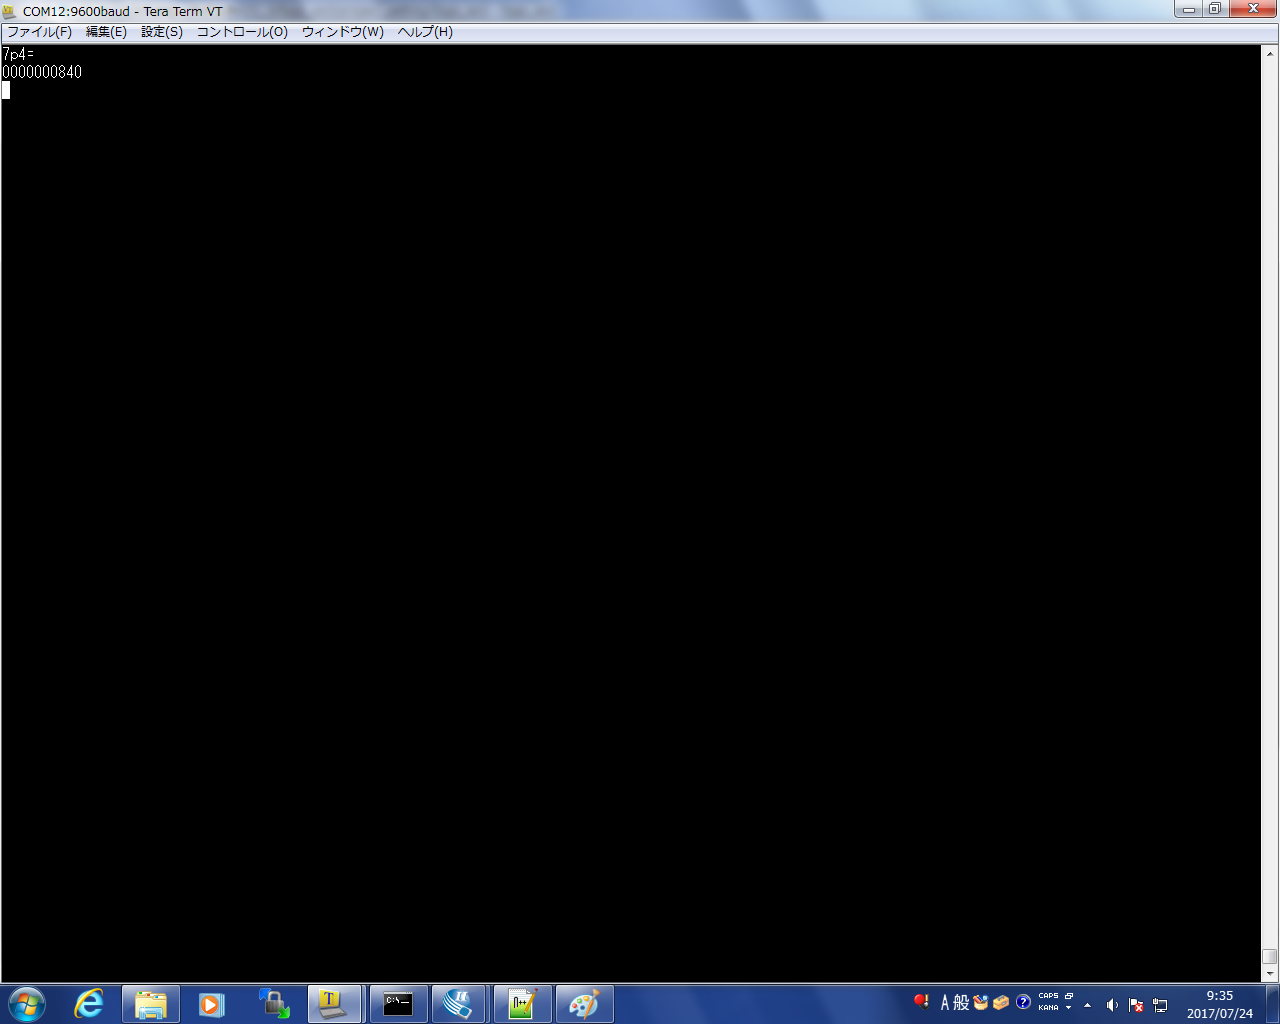
\includegraphics[width=8cm,bb=0 0 1280 1024]{7p4.png}
  \end{center}
  \caption{"$\prod_{i=4}^{7} i=$"}
 \end{minipage}
\end{figure}

\newpage

\subsection*{各サブルーチンの計算方法について}

\subsubsection*{指数}
まず、サブルーチンの呼び出し前にXの値をEXP\_X、Yの値をEXP\_Yに代入しておく。
サブルーチン内ではMUL命令によってEXP\_Xの値をEXP\_Zにかけるという処理をEXP\_Y回行い、
その結果をEXP\_RESに格納する。
かける回数はEXP\_Aをインクリメントすることでカウントし、EXP\_Yとの差が0になったらループを抜ける。
計算終了後、EXP\_A,EXP\_Zを0,1に初期化して、処理を終了する。

\subsubsection*{総乗}
同様に、呼び出し前にX,Yの値をP\_X,P\_Yに代入しておく。
サブルーチン内ではMUL命令によってP\_Yの値をP\_Zにかけていき、かけるごとに
P\_Yの値をインクリメントしている。P\_Yの値がP\_Xに等しくなるとループを抜ける。
計算終了後、P\_Zを1に初期化して処理を終了する。

\subsubsection*{組み合わせ}
同様に、呼び出し前にX,Yの値をC\_X,C\_Yに代入しておく。
サブルーチン内では総乗を計算するサブルーチンPを呼び出している。
P\_Aには$\prod_{i=P\_X-P\_Y+1}^{P\_X} i$を代入し、P\_Bには$P\_Y!$を代入し、
${P\_A}\div{P\_B}$をP\_RESに格納する。
初期化する必要のある変数はないため、計算終了後、処理を終了する。

\subsection*{工夫点}

各計算を処理するサブルーチンの実装において、グローバルに存在するレジスタを利用せず、
それぞれのサブルーチンに入力、出力レジスタを用意し、モジュール化を行った。
サブルーチンの外部とのデータのやり取りは入出力レジスタのみで行い、内部の計算に使用するレジスタはそのサブルーチン内でのみ利用される。
それによって、サブルーチン内で利用するレジスタの初期化をサブルーチン内で行い、再利用可能にすることで、
計算を複数回行う場合や他のサブルーチン内で呼び出しを行えるようにした。
以前作成したプログラムでもサブルーチンをモジュール化することで、容易に再利用可能なサブルーチンを
作るべきだったと感じた。\\
\\



\subsection*{感想}
最初に10進数の入出力を実装する段階で大きく時間を割いてしまい、後半時間が足りなくなってしまった。
前回作成した素数プログラムにおいて10進数の出力を実装していたので、それを利用すれば簡単に実装できると思ったが、
実際は32ビットに対応させたり、整合をとるためにレジスタを変更したりと、計画以上に時間がかかってしまった。
計算機能の追加については、ハードウェア側で乗算と除算を実装してもらえたため、コードを簡潔に書くことができ、実装しやすかった。
また、今回はハードウェアとソフトウェアで担当を分けて行ったため、ハードウェア側の仕様が変わるごとにバグが発生してし
まい、デバッグが大変だった。今回は二人だったが、人数が増えてプロジェクトが大きくなった場合、今回の計画では対応でき
ないと感じた。





\section*{EX3シミュレータのコード}
\lstinputlisting[caption=common\_asm.h, language=c++]{common_asm.h}
\lstinputlisting[caption=ex3\_asm.cpp, language=c++]{ex3_asm.cpp}
\lstinputlisting[caption=ex3\_asm.h, language=c++]{ex3_asm.h}
\lstinputlisting[caption=ex3\_asm\_def.h, language=c++]{ex3_asm_def.h}

\section*{Verilogコード}
\lstinputlisting[caption=cpu\_ex3.v, language=verilog]{cpu_ex3.v}
\lstinputlisting[caption=cpu\_module.v, language=verilog]{cpu_module.v}
\lstinputlisting[caption=def\_ex3.v, language=verilog]{def_ex3.v}
\lstinputlisting[caption=fpga\_ex3.v, language=verilog]{fpga_ex3.v}

\section*{アセンブリコード}
\lstinputlisting[caption=test\_calc1.asm, language=c]{test_calc1.asm}
\end{document}
